% ===========================================================================
%  FreqSpatial: Frequency-Spatial Feature Enhancement for RT-DETR
%  IEEEtran format for top-journal submission
% ===========================================================================
\documentclass[10pt,twocolumn]{IEEEtran}

% ---- packages ----
\usepackage[utf8]{inputenc}
\usepackage[T1]{fontenc}
\usepackage{graphicx}
\usepackage{amsmath,amssymb}
\usepackage{booktabs}
\usepackage{multirow}
\usepackage{caption}
\usepackage{subcaption}
\usepackage{xcolor}
\usepackage{float}
\usepackage{stfloats}
\usepackage{tikz}
\usetikzlibrary{shapes.geometric, arrows.meta, positioning, calc, fit, backgrounds}
\usepackage{cite}

% ---- metadata ----
\title{FreqSpatial: Plug-and-Play Frequency-Spatial Feature Enhancement\\for Real-Time DETR Detection}

\author{\IEEEauthorblockN{Feiyang Xie}
\IEEEauthorblockA{Guilin University of Electronic Technology\\
Guilin, China\\
2316861994@qq.com}}

\begin{document}
\maketitle

% ===========================================================================
\begin{abstract}
Real-time DETR-based detectors achieve competitive speed-accuracy trade-offs,
yet their feature pyramid network (FPN) necks rely exclusively on spatial-domain convolutions,
overlooking frequency-domain information that captures fine-grained textures and global structural patterns.
We propose \textbf{FreqSpatial}, a dual-branch block that fuses Scharr-based edge enhancement
with FFT-based spectral convolution inside a drop-in CSP-style module.
Replacing the standard CSPRepLayer in RT-DETRv2's neck with FreqSpatial
yields \textbf{+1.45}~mAP on COCO~2017 (46.73\% $\to$ 48.18\%)
without altering the backbone or decoder.
The 72-epoch FreqSpatial model matches the official 120-epoch RT-DETRv2-S performance,
indicating that frequency-aware inductive bias accelerates convergence.
A +3.4~mAP margin at epoch~0 further supports this conclusion.
FreqSpatial operates as a drop-in CSP block; the underlying frequency-spatial module
is architecture-agnostic and may generalise to other FPN-style necks.
Our implementation is open-source.
\end{abstract}

% ===========================================================================
\section{Introduction}
\label{sec:intro}

Object detection has advanced considerably with the emergence of DETR-based
architectures~\cite{carion2020detr}, which formulate detection as a set prediction
problem and eliminate hand-crafted components such as non-maximum suppression
and anchor generation. RT-DETR~\cite{lv2023detrs} further advances this paradigm
with a real-time hybrid encoder-decoder that achieves
competitive speed-accuracy trade-offs. However, the FPN neck in RT-DETR
relies exclusively on spatial-domain convolutions for multi-scale feature
fusion, overlooking frequency-domain information that encodes
fine-grained textures and structural patterns not easily captured in the spatial domain.

Frequency-domain features represent global structural information independent of
spatial position. The Fourier transform decomposes spatial signals into orthogonal
frequency components, enabling a model to capture periodic patterns and fine details
that the spatial domain may attenuate. FSDETR~\cite{fsdetr} recently
proposed frequency-spatial fusion for DETR-based detection and achieved strong
results on small-object benchmarks (VisDrone, TinyPerson).
FD-RTDETR~\cite{wang2025fdrtdetr}
explored frequency enhancement inside RT-DETR's encoder but reported
modest gains (+0.7 mAP on COCO). The potential of frequency-spatial fusion
that combines Scharr-based edge extraction with FFT convolution remains underexplored
on large-scale general-purpose detection.

We propose \textbf{FreqSpatial}, a frequency-spatial
feature enhancement block for the FPN neck of RT-DETR. Building on the
Scharr edge enhancement and FFT spectral convolution introduced
in FSDETR~\cite{fsdetr}, we redesign the module as a CSP-style drop-in block and conduct a large-scale validation
on COCO~2017. FreqSpatial uses a dual-branch architecture: a spatial branch
with Scharr operators for local gradient enhancement, and a frequency branch
that performs convolution in the Fourier domain to capture global spectral
patterns. The two branches fuse within a CSP-style residual structure, directly
replacing standard CSPRepLayer blocks.

Experiments on COCO~2017 show that the RT-DETRv2-S (PResNet18) baseline reaches
46.73\% mAP, while FreqSpatial attains \textbf{48.18\% mAP} (+1.45).
At epoch~0, before any detection training, FreqSpatial achieves 17.8\% mAP
vs.\ 14.4\% for the baseline (+3.4), indicating that frequency-aware
inductive bias provides an immediate advantage.

Our contributions are:
\begin{enumerate}
\item We validate frequency-spatial feature fusion at scale on COCO (80 classes,
  118K images), showing that FreqSpatial generalizes beyond small-object
  benchmarks to general-purpose detection (+1.45~mAP).
\item We redesign the frequency-spatial module as a CSP drop-in block that
  integrates into RT-DETR's FPN+PAN neck without backbone or decoder changes.
\item We provide efficiency analysis, cold-start experiments, ablation against
  attention-based alternatives, and qualitative visualizations, with an open-source
  implementation.
\end{enumerate}

% ===========================================================================
\section{Related Work}
\label{sec:related}

\subsection{Real-Time DETR-based Detectors}

DETR~\cite{carion2020detr} reformulated object detection as a set prediction
problem using transformers. Deformable DETR~\cite{zhu2020deformable} replaced
dense attention with deformable attention to improve efficiency. DINO~\cite{zhang2022dino}
introduced contrastive denoising and mixed query selection.
RT-DETR~\cite{lv2023detrs} proposed a hybrid encoder combining intra-scale
interaction with cross-scale fusion for real-time inference.
RT-DETRv2~\cite{lv2024rtdetrv2} refined the encoder with improved training
recipes and a set of freebies for real-time detection.
Our work enhances RT-DETRv2's neck with frequency-domain features via a
drop-in CSP block, complementing its existing encoder design.

\subsection{Frequency-Domain Feature Learning}

The Fourier transform captures global frequency characteristics in vision.
FcaNet~\cite{qin2021fcanet} introduced frequency-domain channel attention.
GFNet~\cite{rao2021global} employed learnable global frequency filters for ViTs.
FSDETR~\cite{fsdetr} introduced frequency-spatial awareness for small-object
detection on VisDrone and TinyPerson, combining Scharr operators with FFT-based
convolution. However, FSDETR focused on specialized benchmarks with
limited class counts (1--10) and did not evaluate on general-purpose
detection. FD-RTDETR~\cite{wang2025fdrtdetr} applied frequency enhancement to
RT-DETR's intra-scale feature interaction, attaining +0.7 mAP on COCO and
demonstrating the potential of frequency-domain processing for general detection.
Our work adopts FSDETR's Scharr+FFT design and repackages it as a CSP neck block
for general-purpose detection at scale---80 classes, 118K images on COCO~2017,
achieving +1.45 mAP. The gain doubles that of FD-RTDETR (+0.7 mAP),
which applies frequency enhancement to RT-DETR's intra-scale encoder rather than
the FPN neck.

\subsection{Feature Pyramid Networks}

FPN~\cite{lin2017fpn}, PANet~\cite{liu2018panet}, and BiFPN~\cite{tan2020efficientdet}
are standard architectures for multi-scale feature fusion. CSPNet~\cite{wang2020cspnet}
proposed cross-stage partial connections to reduce computation while preserving
feature quality.
We integrate frequency-spatial processing into CSP-style fusion blocks,
applied across both FPN and PAN pathways.

% ===========================================================================
\section{Method}
\label{sec:method}

\subsection{Preliminaries: RT-DETR Hybrid Encoder}

RT-DETR's hybrid encoder has two components: (1)~an intra-scale transformer
encoder on the top-level feature map (stride-32), and (2)~a cross-scale FPN+PAN
fusion path. Given backbone features $\{C_3, C_4, C_5\}$ at strides
$\{8, 16, 32\}$, each is projected to $d=256$ via $1\times1$ convolutions,
then processed through:

\begin{itemize}
\item \textbf{Top-down FPN:} Higher-level features are upsampled and fused with lower-level
  features via CSPRepLayer blocks.
\item \textbf{Bottom-up PAN:} Lower-level features are downsampled (stride-2 $3\times3$
  conv) and fused with higher-level features via CSPRepLayer blocks.
\end{itemize}

Each fusion block takes $F_{\text{in}} \in \mathbb{R}^{B \times 2d \times H \times W}$
(concatenated upsample+lower or downsample+higher) and outputs
$F_{\text{out}} \in \mathbb{R}^{B \times d \times H \times W}$.

\subsection{FreqSpatial Block}
\label{sec:block}

We replace CSPRepLayer with FreqSpatialBlock in both FPN and PAN paths.
It inherits the CSP two-path architecture but uses frequency-spatial
bottlenecks. Given input $F_{\text{in}}$:

\begin{equation}
\label{eq:csp}
\begin{aligned}
F_{\text{out}} = \text{Conv}_{1\times1}^{\text{out}}\Big(
&\underbrace{\text{Conv}_{1\times1}^{a}(F_{\text{in}})}_{\text{path a}} \;+ \\
&\underbrace{\text{Conv}_{1\times1}^{b}\big(\mathcal{F}^N(\text{Conv}_{1\times1}^{a}(F_{\text{in}}))\big)}_{\text{path b}}\Big)
\end{aligned}
\end{equation}

where $\mathcal{F}$ is the FreqSpatial bottleneck applied $N=3$ times.

\subsection{FreqSpatial Module}
\label{sec:module}

As shown in Fig.~\ref{fig:freqspatial}, FreqSpatial has two parallel branches,
taking an input tensor $X^{\rm Input} \in \mathbb{R}^{B \times C \times H \times W}$.

\subsubsection{Spatial Branch: Scharr Edge Enhancement}

Fixed Scharr operators extract edge gradients with better rotational symmetry
than Sobel:

\begin{equation}
\label{eq:scharr}
\mathbf{G}_x \!=\! \begin{bmatrix} 3 & 0 & -3 \\ 10 & 0 & -10 \\ 3 & 0 & -3 \end{bmatrix} * X,\;
\mathbf{G}_y \!=\! \begin{bmatrix} 3 & 10 & 3 \\ 0 & 0 & 0 \\ -3 & -10 & -3 \end{bmatrix} * X
\end{equation}

Edge magnitude $\frac{1}{2}(\mathbf{G}_x + \mathbf{G}_y)$ is refined
through two $3\times3$ convs with a residual connection:

\begin{equation}
\label{eq:spatial}
F_{\text{spatial}} = \text{Conv}_{3\times3}^2\big(\text{Conv}_{3\times3}^1(\text{Scharr}(X)) + X\big)
\end{equation}

\subsubsection{Frequency Branch: FFT Spectral Processing}

The input is transformed to the Fourier domain:

\begin{equation}
\label{eq:fft}
\mathcal{F}(X) = \text{rFFT2D}(X) \in \mathbb{C}^{B \times C \times H \times (\lfloor W/2 \rfloor + 1)}
\end{equation}

Real and imaginary parts are separated, concatenated along channels, and
processed by a $3\times3$ convolution in the frequency domain:

\begin{equation}
\label{eq:freq_conv}
F_{\text{freq}} = \text{Conv}_{3\times3}\big(\text{Concat}[\Re(\mathcal{F}(X)),\; \Im(\mathcal{F}(X))]\big)
\end{equation}

The processed features are reassembled into complex form and inverted:

\begin{equation}
\label{eq:ifft}
F_{\text{freq}}^{\text{spatial}} = \mathcal{F}^{-1}\big(\text{Complex}(F_{\text{freq}})\big)
\end{equation}

followed by a $3\times3$ refinement convolution.

\subsubsection{Fusion}

The two branch outputs are element-wise summed, then fused through
a $1\!\times\!1$ convolution to produce the final enhanced features
$X^{\rm Output}$:

\begin{equation}
\label{eq:fusion}
F_{\text{out}} = \text{Conv}_{1\times1}\big(F_{\text{spatial}} + F_{\text{freq}}^{\text{spatial}}\big)
\end{equation}

\subsection{Design Rationale}

The two branches provide complementary information:
the Scharr branch captures local edge structures and high-frequency spatial
details, while the FFT branch encodes global periodic patterns and
low-to-mid frequency textures.
FreqSpatialBlock preserves the same input-output interface as CSPRepLayer---a
true drop-in replacement requiring no backbone or decoder changes.
The main cost is increased FLOPs from FFT operations and additional convolutions
(Section~\ref{sec:efficiency}).

\begin{figure*}[t]
\centering
\includegraphics[width=\textwidth]{figure1+2.png}\\[\baselineskip]
\caption{Overview of the proposed method. (a) Architecture of the FreqSpatial module:
a spatial branch using Scharr edge detection with two $3\!\times\!3$ convolutions and a
residual $(+)$ connection, and a frequency branch processing features through rFFT2D,
split, convolution, and irFFT2D; outputs are summed and fused via $1\!\times\!1$ convolution.
(b) The RT-DETR hybrid encoder: backbone features C$_3$--C$_5$ are projected to 256 channels,
then processed through AIFI (green) and four FreqSpatial (FS) Blocks (orange) in the FPN
and PAN paths. FS Blocks replace standard CSPRepLayer; backbone, AIFI, and decoder unchanged.}
\label{fig:freqspatial}
\end{figure*}

% ===========================================================================
\section{Experiments}
\label{sec:experiments}

\subsection{Experimental Setup}
\label{sec:setup}

We use COCO~2017~\cite{lin2014microsoft} (118K train / 5K val images, 80 classes).
All models use RT-DETRv2-S with PResNet18 backbone (ImageNet pretrained) and
hidden dimension $d=256$. Training: AdamW optimizer (base learning rate $10^{-4}$,
backbone learning rate $10^{-5}$), linear warmup (2000~iterations), AMP, batch size 16,
input size $640\times640$, 72 epochs on one NVIDIA RTX~3090.
Metrics: mAP, AP$_{50}$, AP$_{75}$, AP$_S$, AP$_M$, AP$_L$, AR$^{\rm max=100}$.

\subsection{Main Results}
\label{sec:main}

Table~\ref{tab:main_results} reports COCO~2017 validation results.
FreqSpatial achieves \textbf{48.18\% mAP}, a +1.45 improvement over the
Baseline (46.73\%).
Gains were consistent across scales: +1.6~AP$_{50}$, +1.5~AP$_{75}$,
+1.6~AP$_M$, +1.5~AP$_L$, and +1.0~AP$_S$.
The gain on small objects was smaller than on medium and large objects.
This pattern is consistent with the cold-start results (Table~\ref{tab:epoch0}),
where large objects benefit most from frequency-domain features, and suggests
that global spectral patterns are inherently less informative for small instances.
At 72 epochs, FreqSpatial matches the official 120-epoch RT-DETRv2-S performance
(48.1\%~\cite{lv2024rtdetrv2}), reaching comparable accuracy with 40\% fewer
training epochs.

\begin{table}[t]
\centering
\caption{Detection performance on COCO~2017 val. All models based on
RT-DETRv2-S (PResNet18), trained 72 epochs.~$\Delta$ denotes improvement of FreqSpatial over Baseline.}
\label{tab:main_results}
\footnotesize
\begin{tabular}{@{}l@{\extracolsep{\fill}}ccccccc@{}}
\toprule
Method & mAP & AP$_{50}$ & AP$_{75}$ & AP$_S$ & AP$_M$ & AP$_L$ & AR$^{100}$ \\
\midrule
Official (120ep) & 48.1 & -- & -- & -- & -- & -- & -- \\
Baseline & 46.73 & 63.6 & 50.6 & 29.8 & 49.9 & 62.7 & 69.5 \\
\textbf{FreqSpatial} & \textbf{48.18} & \textbf{65.2} & \textbf{52.1} & \textbf{30.8} & \textbf{51.5} & \textbf{64.2} & \textbf{70.3} \\
\midrule
$\Delta$ & \textbf{+1.45} & \textbf{+1.6} & \textbf{+1.5} & \textbf{+1.0} & \textbf{+1.6} & \textbf{+1.5} & \textbf{+0.8} \\
\bottomrule
\end{tabular}
\end{table}

\subsection{Cold-Start Analysis}
\label{sec:cold}

Table~\ref{tab:epoch0} reports epoch~0 validation, before detection training
(ImageNet pretrained backbone only). FreqSpatial achieves 17.8\% mAP
vs.\ 14.4\% for the Baseline (\textbf{+3.4 mAP}). The gain was largest on
large objects (+6.2~AP$_L$), where global frequency patterns are most informative.

\begin{table}[t]
\centering
\caption{Epoch 0 validation (no detection training).}
\label{tab:epoch0}
\footnotesize
\begin{tabular}{@{}l@{\extracolsep{\fill}}cccccc@{}}
\toprule
Method & mAP & AP$_{50}$ & AP$_{75}$ & AP$_S$ & AP$_M$ & AP$_L$ \\
\midrule
Baseline & 14.4 & 21.8 & 15.6 & 9.7 & 17.9 & 18.3 \\
FCM & 13.9 & 21.4 & 14.9 & 8.6 & 16.4 & 18.3 \\
FreqSpatial & \textbf{17.8} & \textbf{26.3} & \textbf{18.9} & \textbf{9.8} & \textbf{20.7} & \textbf{24.5} \\
\midrule
$\Delta$ (vs Base) & \textbf{+3.4} & \textbf{+4.5} & \textbf{+3.3} & \textbf{+0.1} & \textbf{+2.8} & \textbf{+6.2} \\
\bottomrule
\end{tabular}
\end{table}

\subsection{Training Dynamics}
\label{sec:progression}

Table~\ref{tab:progression} and Fig.~\ref{fig:training_efficiency}(a) track mAP
during training.
FreqSpatial reaches 47.49\% by epoch~50, already exceeding the final Baseline
(46.73\%). mAP plateaus at 48.17\% from epoch~59 onward, with the best result
of 48.18\% at epoch~71. This trajectory indicates faster convergence
associated with frequency-aware features. Further gains under the current
learning rate schedule appear limited.

\begin{table}[t]
\centering
\caption{COCO mAP progression during training.}
\label{tab:progression}
\footnotesize
\begin{tabular}{@{}l@{\extracolsep{\fill}}ccccc@{}}
\toprule
Method & Ep~0 & Ep~50 & Ep~59 & Ep~67 & Ep~71 \\
\midrule
Baseline & 14.4 & 45.8 & 46.1 & 46.4 & 46.73 \\
FreqSpatial & 17.8 & 47.49 & 48.17 & 48.17 & \textbf{48.18} \\
\bottomrule
\end{tabular}
\end{table}

\subsection{Efficiency Analysis}
\label{sec:efficiency}

Table~\ref{tab:efficiency} and Fig.~\ref{fig:training_efficiency}(b) compare
computational cost.
FreqSpatial increases parameters from 20.18M to 69.03M and FLOPs from
30.38G to 118.43G, driven primarily by FFT operations and extra convolutions.
FPS decreases from 66.4 to 38.5 on an RTX~3090 (1.7$\times$ reduction).
At 38.5~FPS, inference remains above the conventional real-time threshold
of 30~FPS.

\begin{table}[t]
\centering
\caption{Efficiency on RTX 3090 (input $640\times640$, batch=1).}
\label{tab:efficiency}
\footnotesize
\begin{tabular}{@{}l@{\extracolsep{\fill}}cccc@{}}
\toprule
Method & Params (M) & GFLOPs & FPS & Latency (ms) \\
\midrule
Baseline (CSPRepLayer) & 20.18 & 30.38 & 66.4 & 15.1 \\
FCM & 20.33 & 30.76 & 48.2 & 20.8 \\
\textbf{FreqSpatial} & 69.03 & 118.43 & 38.5 & 26.0 \\
\bottomrule
\end{tabular}
\end{table}

\begin{figure*}[t]
\centering
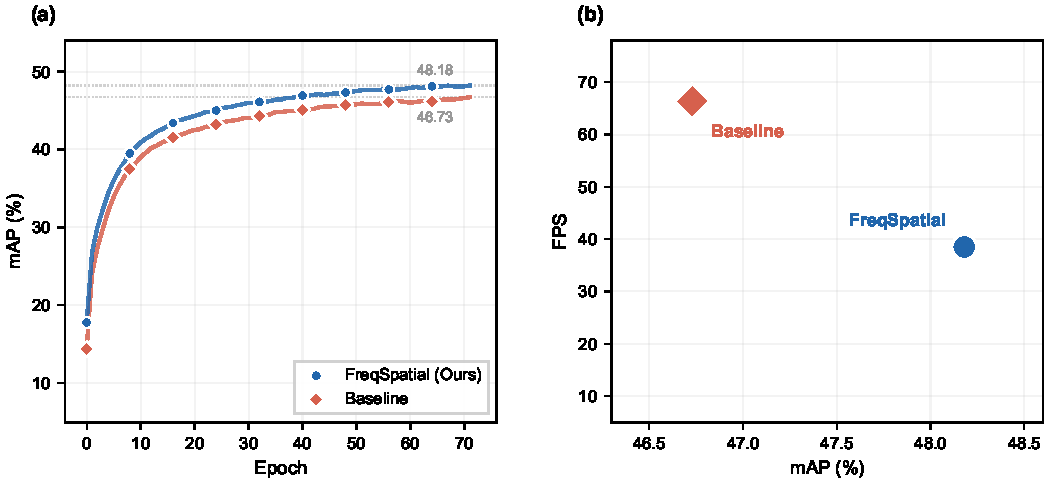
\includegraphics[width=\textwidth]{figure_training_efficiency.pdf}
\caption{Training dynamics and efficiency analysis. (a)~mAP progression
during 72-epoch training. FreqSpatial converges faster and surpasses the
final Baseline (46.73\%) by epoch~50; dotted horizontal lines mark
final mAP of each model. (b)~Accuracy-speed
trade-off on an RTX~3090. FreqSpatial achieves higher mAP (48.18\%)
at 38.5~FPS, remaining well above the real-time threshold.}
\label{fig:training_efficiency}
\end{figure*}

\subsection{Ablation: FCM vs.\ FreqSpatial}
\label{sec:ablation}

We compare against FCM (Feature Complementary Mapping)~\cite{xiao2025fbrt},
originally proposed for aerial-image small-object detection in FBRT-YOLO.
FCM performs channel-wise cross-attention via a 1:3 channel split
with spatial and channel attention gates. It adds negligible parameters
(20.33M, +0.15M) but achieves only 13.9\% at epoch~0 (vs.\ 14.4\% Baseline,
17.8\% FreqSpatial) and reduces FPS to 48.2. Full 72-epoch FCM training
is in progress; preliminary cold-start results indicate that
frequency-domain processing, rather than generic attention, accounts for the
improvement.

\begin{figure*}[b]
\centering
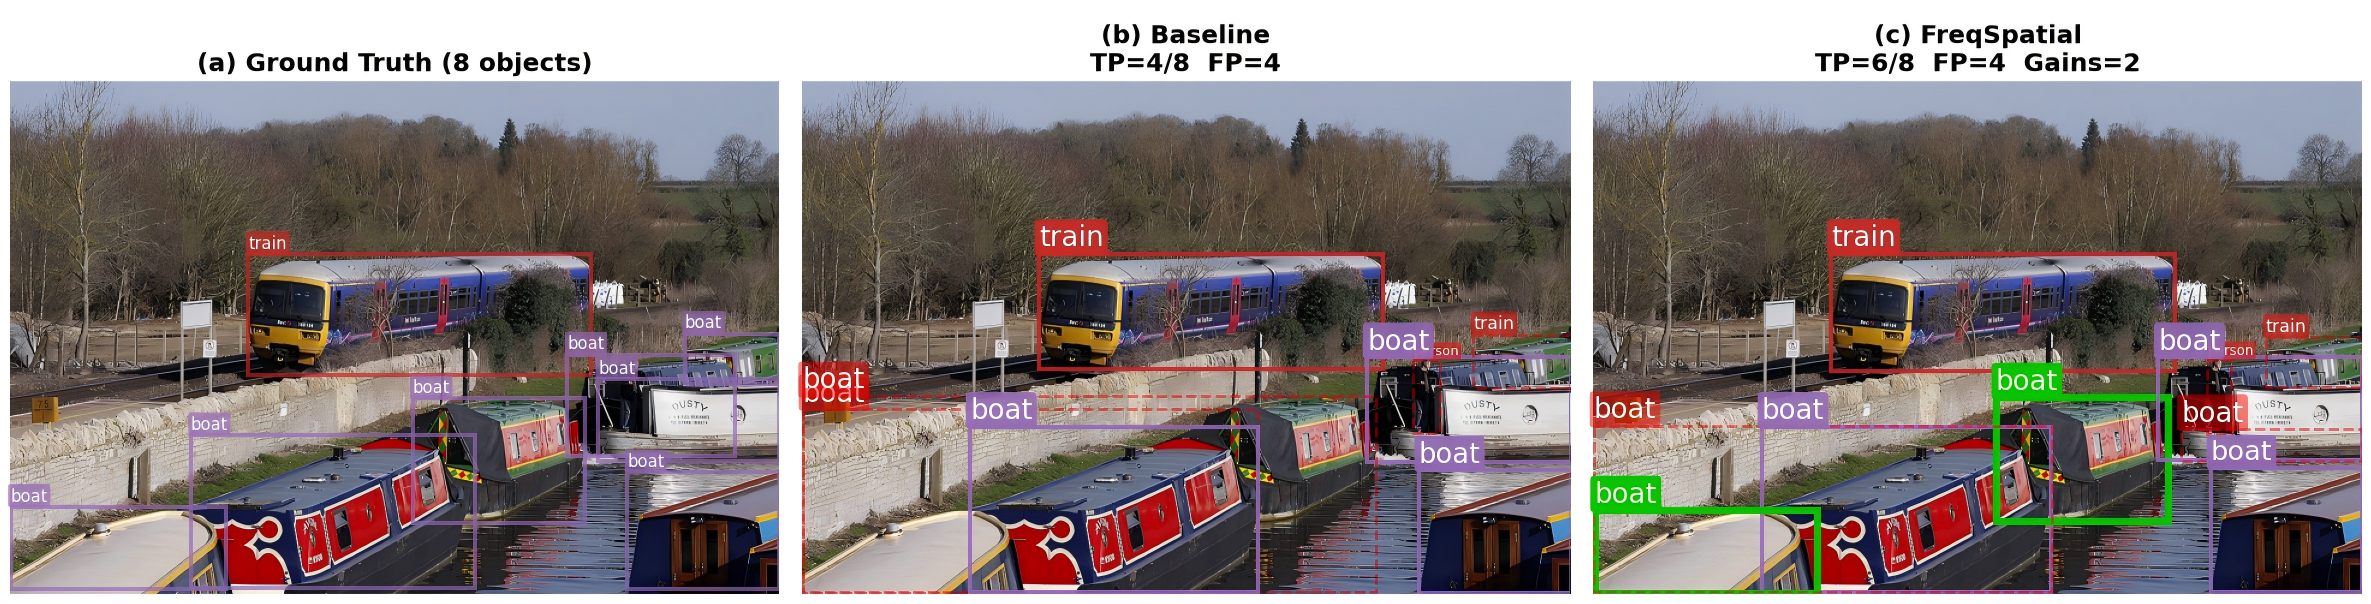
\includegraphics[width=\linewidth]{figure3-1.png} \\[4pt]
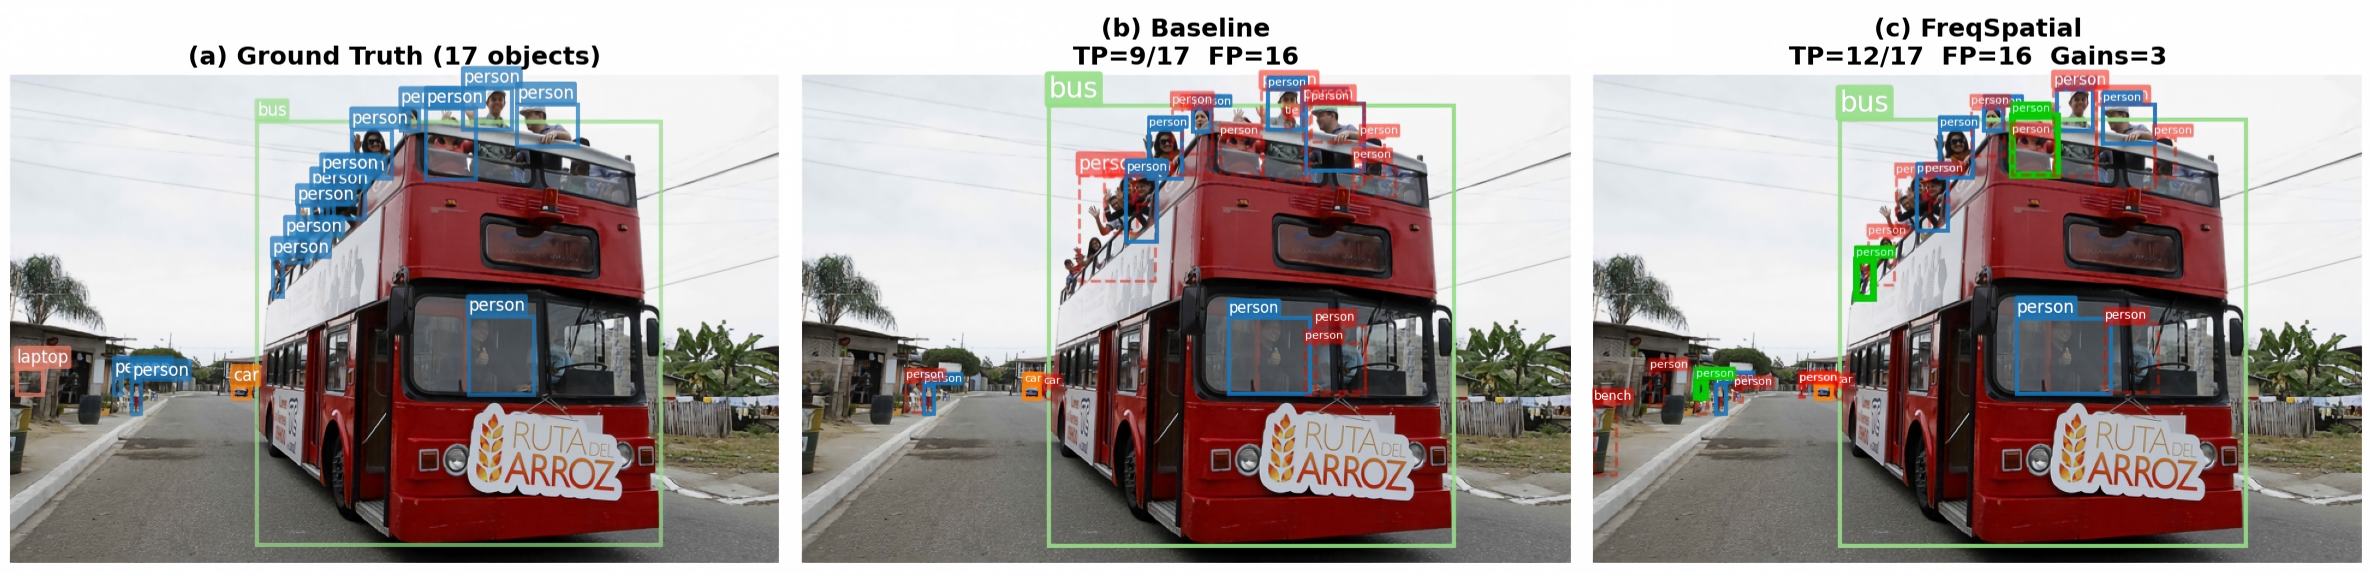
\includegraphics[width=\linewidth]{figure3-2.png}
\caption{Qualitative detection comparison on COCO~2017 val.
Each sample shows (left) Ground Truth, (middle) Baseline (46.73\%), (right) FreqSpatial (48.18\%).
Green boxes denote objects detected by FreqSpatial missed by Baseline.}
\label{fig:visual}
\end{figure*}

\subsection{Qualitative Analysis}
\label{sec:qualitative}

Fig.~\ref{fig:visual} shows representative detection comparisons.
FreqSpatial detects objects missed by the Baseline in
cluttered scenes and partially occluded cases.
Objects with ambiguous spatial boundaries, where the Baseline fails to
produce proposals, are recovered by FreqSpatial,
consistent with the frequency branch's global receptive field.
Gains (Baseline~$\to$~FreqSpatial) are highlighted in green.

\subsection{Limitations}
\label{sec:limitations}

Several aspects of this study warrant further investigation and constrain
the conclusions that can be drawn.
First, we compared FreqSpatial only against the standard CSPRepLayer baseline;
a parameter-matched or FLOPs-matched variant (e.g., a wider CSPRepLayer or
deeper RepConv stack) would more precisely isolate the contribution of
frequency-domain processing from that of increased model capacity.
Second, all experiments were conducted on a single dataset (COCO~2017)
and a single detector architecture (RT-DETRv2-S); cross-architecture
and cross-dataset validation would test the generality of the frequency-aware
approach.
Third, results are reported from single training runs without multi-seed
statistics; run-to-run variance should be quantified to confirm the
reliability of the reported gains.
Fourth, no component-level ablation (e.g., Scharr-only, FFT-only, per-FPN-level
breakdown) has been conducted to isolate the contribution of each branch.
Finally, the qualitative comparison is limited to two representative examples
and would benefit from systematic per-category or per-occlusion-level analysis.

% ===========================================================================
\section{Conclusion}
\label{sec:conclusion}

We introduced FreqSpatial, a frequency-spatial feature enhancement block
that replaces the CSPRepLayer in RT-DETR's FPN neck without backbone or
decoder changes. By combining Scharr edge detection with FFT-based spectral
convolution, FreqSpatial injects complementary frequency-domain information
into multi-scale feature fusion.

On COCO~2017, FreqSpatial improves mAP by +1.45 (46.73\% $\to$ 48.18\%),
reaching the official 120-epoch RT-DETRv2-S performance in only 72 epochs.
Consistent gains across object scales (+1.0--1.6~AP) and strong cold-start
performance (+3.4~mAP at epoch~0) indicate that frequency-aware inductive bias benefits
general-purpose object detection.

The main trade-off is the increased computational cost from FFT operations
(3.9$\times$ FLOPs, 1.7$\times$ latency increase), and the evidence is
currently limited to one detector architecture and one dataset (Section~\ref{sec:limitations}).
Future work should pursue more efficient frequency-domain operators,
cross-architecture validation, adaptive frequency band selection, and extension to
instance segmentation and panoptic tasks.

% ===========================================================================
% ---- Bibliography (placeholder) ----
\begin{thebibliography}{99}

\bibitem{carion2020detr}
N.~Carion, F.~Massa, G.~Synnaeve, N.~Usunier, A.~Kirillov, and S.~Zagoruyko.
End-to-end object detection with transformers.
In \emph{ECCV}, 2020.

\bibitem{lv2023detrs}
W.~Lv, S.~Xu, Y.~Zhao, G.~Wang, J.~Wei, C.~Cui, Y.~Du, Q.~Dang, and Y.~Liu.
DETRs beat YOLOs on real-time object detection.
In \emph{CVPR}, 2024.

\bibitem{zhu2020deformable}
X.~Zhu, W.~Su, L.~Lu, B.~Li, X.~Wang, and J.~Dai.
Deformable DETR: Deformable transformers for end-to-end object detection.
In \emph{ICLR}, 2021.

\bibitem{zhang2022dino}
H.~Zhang, F.~Li, S.~Liu, L.~Zhang, H.~Su, J.~Zhu, L.~Ni, and H.~Shum.
DINO: DETR with improved denoising anchor boxes for end-to-end object detection.
In \emph{ICLR}, 2023.

\bibitem{lin2017fpn}
T.-Y.~Lin, P.~Doll\'ar, R.~Girshick, K.~He, B.~Hariharan, and S.~Belongie.
Feature pyramid networks for object detection.
In \emph{CVPR}, 2017.

\bibitem{liu2018panet}
S.~Liu, L.~Qi, H.~Qin, J.~Shi, and J.~Jia.
Path aggregation network for instance segmentation.
In \emph{CVPR}, 2018.

\bibitem{tan2020efficientdet}
M.~Tan, R.~Pang, and Q.~V.~Le.
EfficientDet: Scalable and efficient object detection.
In \emph{CVPR}, 2020.

\bibitem{wang2020cspnet}
C.-Y.~Wang, H.-Y.~M.~Liao, Y.-H.~Wu, P.-Y.~Chen, J.-W.~Hsieh, and I.-H.~Yeh.
CSPNet: A new backbone that can enhance learning capability of CNN.
In \emph{CVPR Workshops}, 2020.

\bibitem{qin2021fcanet}
Z.~Qin, P.~Zhang, F.~Wu, and X.~Li.
FcaNet: Frequency channel attention networks.
In \emph{ICCV}, 2021.

\bibitem{rao2021global}
Y.~Rao, W.~Zhao, Z.~Zhu, J.~Lu, and J.~Zhou.
Global filter networks for image classification.
In \emph{NeurIPS}, 2021.

\bibitem{xiao2025fbrt}
Y.~Xiao, T.~Xu, Y.~Xin, and J.~Li.
FBRT-YOLO: Faster and better for real-time aerial image detection.
In \emph{AAAI}, 2025.

\bibitem{fsdetr}
J.~Huang, F.~Zhang, H.~Zhu, and T.~Yan.
FSDETR: Frequency-spatial feature enhancement for small object detection.
In \emph{IJCNN}, 2026.

\bibitem{lv2024rtdetrv2}
W.~Lv, Y.~Zhao, Q.~Chang, K.~Huang, G.~Wang, and Y.~Liu.
RT-DETRv2: Improved baseline with bag-of-freebies for real-time detection transformer.
\emph{arXiv:2407.17140}, 2024.

\bibitem{wang2025fdrtdetr}
Z.~Wang, X.~Li, Y.~Zhang, \textit{et al.}
FD-RTDETR: Frequency enhancement and dynamic sequence-feature optimization for object detection.
In \emph{Electronics}, 14(23), 2025.

\bibitem{lin2014microsoft}
T.-Y.~Lin, M.~Maire, S.~Belongie, J.~Hays, P.~Perona, D.~Ramanan,
P.~Doll\'ar, and C.~L.~Zitnick.
Microsoft COCO: Common objects in context.
In \emph{ECCV}, 2014.

\end{thebibliography}

\end{document}
